\documentclass[9pt]{beamer}
\usepackage[sfdefault]{roboto}
\usepackage{styles/fluxmacros}
\usefolder{styles}
\usetheme[style=asphalt]{flux}
\usepackage{xcolor}
\usepackage{color}
\usepackage{colortbl}
\usepackage{amsmath}
\usepackage{amssymb}
\usepackage{graphicx}
\usepackage{latexsym}
\usepackage[T1]{fontenc}
\usepackage[utf8]{inputenc}
\usepackage{wrapfig}
\usepackage{siunitx}
\usepackage{times}
\usepackage{tikz}
\usepackage{verbatim}
\usepackage{multimedia}
\usepackage{hyperref}
\usepackage{thumbpdf}
\usepackage{pgf,pgfarrows,pgfnodes,pgfautomata,pgfheaps,pgfshade}
\usepackage{url}
\usepackage{empheq}
\usepackage{fancybox}
\usepackage{esint}
\usepackage{lipsum}
\usepackage{listings}
\usepackage{mathptmx}
\usepackage{helvet}
\usepackage{tikz}%
\usepackage{circuitikz}
\usepackage{csvsimple}
\usepackage{pgfplots}
\usepackage{multimedia}
\usepackage{media9}
\usepackage{proba}
\usepackage[absolute,overlay]{textpos}
\usepackage{bibunits}
\usepackage{tcolorbox}
%\usepackage[texcoord,
%            grid,
%            gridunit=mm,
%            gridcolor=red!60,
%            subgridcolor=black!60]{eso-pic}
\usepackage{enumerate}
\setbeamercovered{transparent}
%% Informations
\usepackage[makeroom]{cancel}
\usepackage{epstopdf}
\epstopdfsetup{outdir=./}
\mode<presentation>
{  
    %\usetheme{PaloAlto}
    %\usecolortheme[named=kugreen]{structure}
    \useinnertheme{progressbar}
    %\usefonttheme{default}
    %\usefonttheme{serif}
    %\setbeamercovered{transparent}
    %\setbeamertemplate{blocks}[rounded][shadow=true]
    %s\setbeamertemplate{navigation symbols}[only frame symbol]
}
   %
%

%~~~~~~~~~~~~~~~~~~~~~~~~~~~~~~~~~~~~~~~~~~~~~~~~~~~~~~~~~~~~~~~~~~~~~~~~~~~~~~

%~~~~~~~~~~~~~~~~~~~~~~~~~~~~~~~~~~~~~~~~~~~~~~~~~~~~~~~~~~~~~~~~~~~~~~~~~~~~~~
% Informations
\title{Modelling SDEs in biology\\
    Formulation, Numerical Simulation and Analysis.}
\subtitle{Second day: Numerical methods for SDEs}
\author{Saúl Díaz Infante Velasco}
\institute{CONACYT-UNIVERSIDAD de SONORA, Cimat, Guanajuato Gto}
\date{\today}
\titlegraphic{assets/background_image.png}
%~~~~~~~~~~~~~~~~~~~~~~~~~~~~~~~~~~~~~~~~~~~~~~~~~~~~~~~~~~~~~~~~~~~~~~~~~~~~~~
%%%%%%%%%%%%%%%%%%%%%%%%%%%%%%%%%%%%%%%%%%%%%%%%%%%%%%%%%%%%%%%%%%%%%%%%%%%%%%%%
\def\Q#1#2{\frac{\partial #1}{\partial #2}}
\usetikzlibrary{arrows,shapes}
\pgfplotsset{compat=1.14}
%%%%%%%%%%%%%%%%%%%%%%%%%%%%%%%%%%%%%%%%%%%%%%%%%%%%%%%%%%%%%%%%%%%%%%%%%%%%%%%%
%------------------------------------Theorems 
\theoremstyle{plain} % default
\newtheorem{Teorema}{Teorema}
\newtheorem{Ejemplo}{Ejemplo}
\theoremstyle{definition}
\newtheorem{Definicion}{Definici\'on}
\newtheorem{Corolario}{Corolario}
\newtheorem{Proposicion}{Proposici\'on}
\newtheorem{Prueba}{Prueba}
\theoremstyle{definition}
\newtheorem{definicion}{Definici\'on}
\newtheorem{lema}{Lema}
%-----------------------------ExtrasDeTercerPresentacion
%--------------------------------Fancyboxes-------------------------------------
\definecolor{myblue}{rgb}{.8, .8, 1}
\definecolor{shadecolor}{cmyk}{0,0,0.41,0}
\newcommand*\mybluebox[1]{%
    \colorbox{myblue}{\hspace{1em}#1\hspace{1em}}
}
\newcommand*\myyellowbox[1]{%
    \colorbox{darkyellow}{\hspace{1em}#1\hspace{1em}}
}
%--------------------------------------------------------------------------
\definecolor{shadecolor}{cmyk}{0,0,0.41,0}
\definecolor{light-blue}{cmyk}{0.25,0,0,0}
\newsavebox{\mysaveboxM} % M for math
\newsavebox{\mysaveboxT} % T for text
\newcommand*\Garybox[2][Example]{%
    \sbox{\mysaveboxM}{#2}%
        \sbox{\mysaveboxT}{\fcolorbox{black}{light-blue}{#1}}%
            \sbox{\mysaveboxM}{%
    \parbox[b][\ht\mysaveboxM+.5\ht\mysaveboxT+.5\dp\mysaveboxT][b]{%
        \wd\mysaveboxM}{#2}%
    }%
    \sbox{\mysaveboxM}{%
        \fcolorbox{black}{shadecolor}{%
        \makebox[\linewidth-10em]{\usebox{\mysaveboxM}}%
        }%
    }%
    \usebox{\mysaveboxM}%
    \makebox[0pt][r]{%
        \makebox[\wd\mysaveboxM][c]{%
            \raisebox{\ht\mysaveboxM-0.5\ht\mysaveboxT
            +0.5\dp\mysaveboxT-0.5\fboxrule}{\usebox{\mysaveboxT}}%
        }%
    }%
}
\newcommand\Fontvi{\fontsize{7}{7.2}\selectfont}
%%%%%%%%%%%%%%%%%%%%%%%%%%%%%%%%%%%%%%%%%%%%
\definecolor{kugreen}{RGB}{50,93,61}
\definecolor{kugreenlys}{RGB}{132,158,139}
\definecolor{kugreenlyslys}{RGB}{173,190,177}
\definecolor{kugreenlyslyslys}{RGB}{214,223,216}
\definecolor{greenArea}{RGB}{124,252,124}
\definecolor{hellmagenta}{rgb}{1,0.75,0.9}
\definecolor{hellcyan}{rgb}{0.75,1,0.9}
\definecolor{hellgelb}{rgb}{1,1,0.8}
\definecolor{colKeys}{rgb}{0,0,1}
\definecolor{colIdentifier}{rgb}{0,0,0}
\definecolor{colComments}{rgb}{1,0,0}
\definecolor{colString}{rgb}{0,0.5,0}
\definecolor{darkyellow}{rgb}{1,0.9,0}
\setbeamercovered{transparent}
\lstset{%
    language=[AlLaTeX]TEX,%
    float=hbp,%
    basicstyle=\ttfamily\small, %\usepackage{cir}
    identifierstyle=\color{colIdentifier}, %
    keywordstyle=\color{colKeys}, %
    stringstyle=\color{colString}, %
    commentstyle=\color{colComments}, %
    columns=flexible, %
    tabsize=3, %
    frame=single, %
    extendedchars=true, %
    showspaces=false, %
    showstringspaces=false, %
    numbers=left, %
    numberstyle=\tiny, %
    breaklines=true, %
    backgroundcolor=\color{hellgelb}, %
    breakautoindent=true, %
    captionpos=b,%
    xleftmargin=18pt,%
    xrightmargin=\fboxsep%
}
\pgfplotsset{
    left segments/.code={\pgfmathsetmacro\leftsegments{#1}},
    left segments=3,
    left/.style args={#1:#2}{
        ybar interval,
        domain=#1:#2,
        samples=\leftsegments+1,
        x filter/.code=\pgfmathparse{\pgfmathresult}
       }
}
\DeclareMathOperator{\sign}{sgn}
\newcommand{\innerprod}[2]{\left\langle#1, #2\right\rangle}
\newcommand\bound{10} % bound number of points on each side of N
\newcommand\labelnum[3][]{
    \begin{scope}[font=\footnotesize,x=.3cm,#1]
      \foreach \mypt in {0,#2,...,\bound}{
        \draw(\mypt,0)circle[radius=2pt];
        \draw(-\mypt,0)circle[radius=2pt];
      }
      \draw(-\bound-5,0)--(\bound+5,0) node[pos=0, left]{$t$};
      \node(start)[at={(-\bound-4,0)},label=below:{$t_0=0$}]{$[$};
      \node(end)[at={(\bound+4,0)},label=below:{$T=Nh$}]{$]$};
      \node[%
          at={($(start)!.319!(end)$)},
          label=below:{
               $\underbrace{}_{h}$
            }%
            ]{\vphantom{$[$}};
      \node[at={($(start)!.57!(end)$)},label=below:{$t_{n+1}$}]{\vphantom{$[$}};
      \filldraw(0,0)circle[radius=2pt];
      \node[at={(-\bound-2,0)},above]{$\cdots$};
      \node[at={(\bound+2,0)},above]{$\cdots$};
      \node[at={(0,0)},above=5pt]{#3};
    \end{scope}
}
\usepackage{remreset}
\makeatletter
\@removefromreset{subsection}{section}
\makeatother
\definecolor{greenstrong}{rgb}{0.58,0.77,0.29}
\definecolor{redstrong}{rgb}{0.81,0.22,0.23}
\definecolor{fglisting}{gray}{0.3}
\definecolor{bglisting}{gray}{1}
\definecolor{fgshell}{gray}{1}
\definecolor{bgshell}{gray}{0.1}
\definecolor{bgshelllight}{gray}{0.8}
%
\setcounter{subsection}{1}
\newcommand{\hl}[1]{\textcolor{greenstrong}{#1}}
\newcommand{\hlErr}[1]{\textcolor{redstrong}{\texttt{#1}}}
\newcommand{\hlOk}[1]{\textcolor{green}{\texttt{#1}}}
\newcommand{\hlInv}[1]{\colorbox{bgshell}{\textcolor{fgshell}{\texttt{#1}}}}
\newcommand{\unhl}[1]{\textcolor{gray}{#1}}
\newcommand{\clda}[0]{$\textcolor{blue}{\lambda}$}
\newcommand{\carr}[0]{$\textcolor{purple}{\rightarrow}$}
\newcommand{\cbind}[0]{\textbf{\texttt{$>\!\!>\!\!=$}}}
\newcommand{\codedots}[0]{\textcolor{mid-gray}{...}}

%
\tcbuselibrary{skins, breakable}
\newtcolorbox{greenbox}[1]{%
        colback = green!5!white,
        colframe = green!55!black,
        fonttitle = \bfseries,
        title = #1 %
    }
\newtcolorbox{bluebox}[1]{%
        colback = blue!5!white,
        colframe = blue!55!black,
        fonttitle = \bfseries,
        title = #1
    }
%
\newtcolorbox{graybox}[1]{%
        colback = gray!5!white,
        colframe = gray!55!black,
        fonttitle = \bfseries,
        title = #1
    }
%
\newtcolorbox{yellowbox}[1]{%
        colback = yellow!5!white,
        colframe = yellow!55!black,
        fonttitle = \bfseries,
        title = #1
    }

\begin{document}
    \titlepage
    \section{HW}
        % \begin{frame}{SIS-DTCM}
%     \begin{center}
%     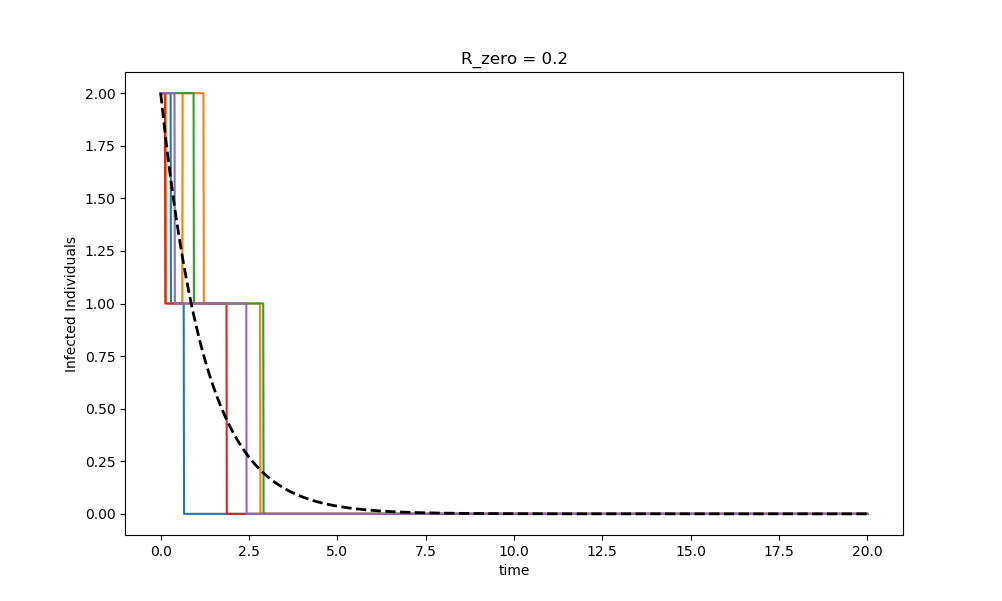
\includegraphics[width=\textwidth]{./homework/HW01.png}
%     % HW01.png: 0x0 pixel, 300dpi, 0.00x0.00 cm, bb=
%     \end{center}
% \end{frame}
%%%%%%%%%%%%%%%%%%%%%%%%%%
\begin{frame}{SIS-CTCM}
    \begin{center}
    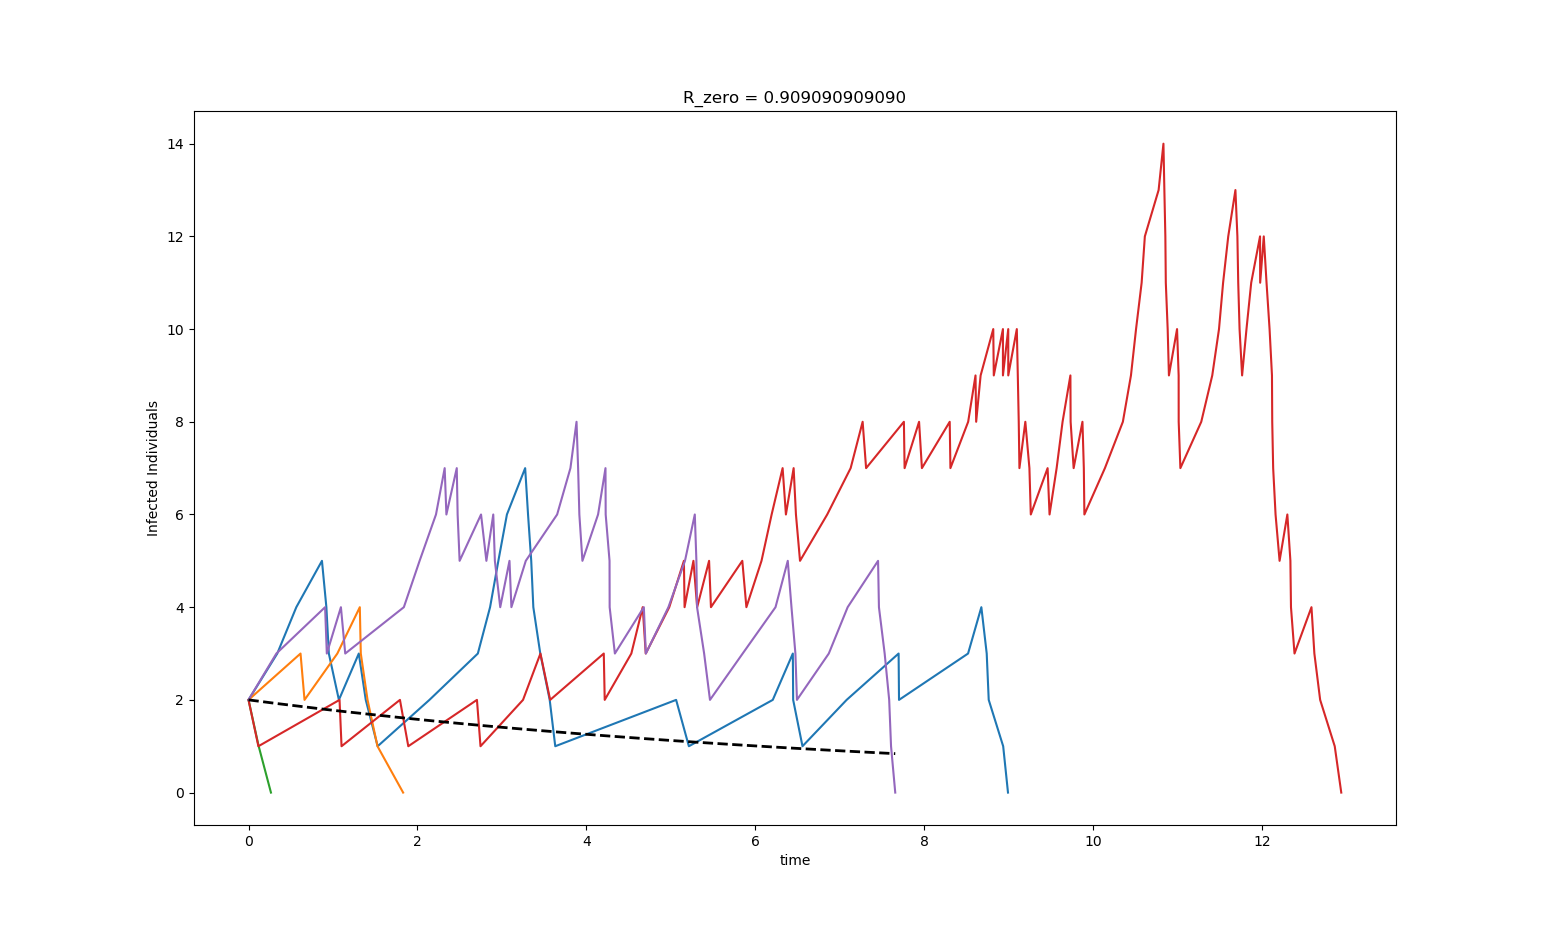
\includegraphics[width=\textwidth]{./homework/HW02.png}
    % HW01.png: 0x0 pixel, 300dpi, 0.00x0.00 cm, bb=
    \end{center}
\end{frame}
% \begin{frame}{SIS-SDE}
%     \begin{center}
%     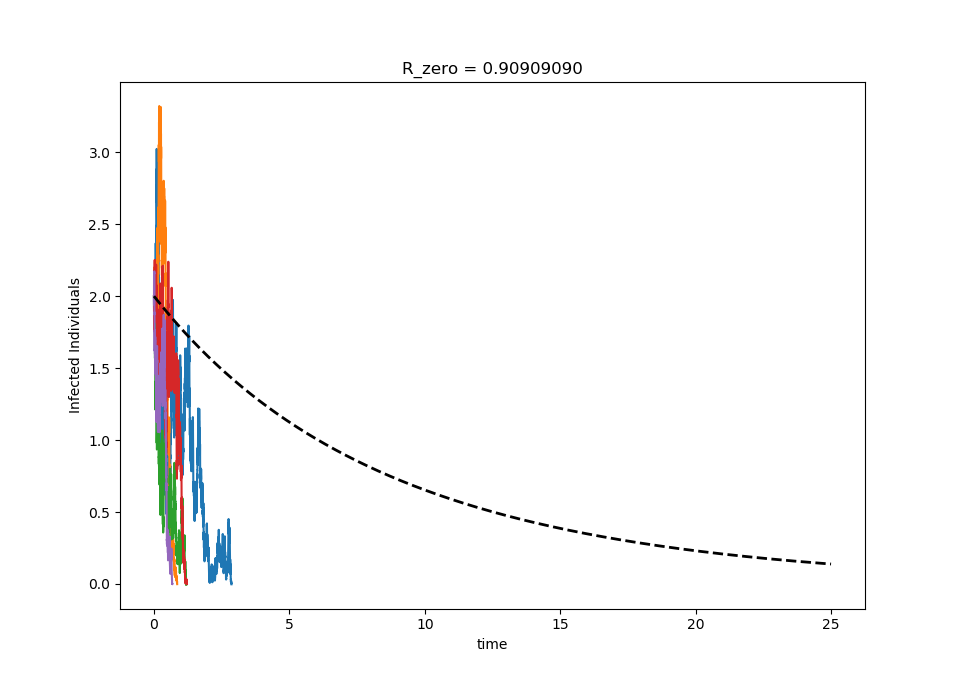
\includegraphics[width=\textwidth]{./homework/HW03.png}
%     % HW01.png: 0x0 pixel, 300dpi, 0.00x0.00 cm, bb=
%     \end{center}
% \end{frame}

    \begin{frame}
        \frametitle{Table of contents}
        \tableofcontents
    \end{frame}
    \section{LM}
        \begin{frame}{}
    Let, $I_t = i$. Denote by $T_i$ the interevent time.
    $H_i(t) \probX{T_i>t}$.
    \begin{align*}
        H_i(t + \Delta t) &= H_i(t) p_{ii}(\Delta t)
        \\
            &=H_i(t)(1 -(b(i) + d(i)) ) \Delta_t + o(\Delta t)
        \\
        \frac{H_i(t + \Delta t) - H_i(t)}{\Delta t } 
            &= -(b(i)+d(i))H_i(t) + o(\Delta t)
    \end{align*}
    Thus
    $$
        \frac{d H_i(t)}{dt} = -(b(i)+d(i))H_i(t)
    $$
    which have solution
    $
        H_i(t) = \exp(-(b(i)+d(i)) t )
    $
\end{frame}
\begin{frame}{}
    Let $F_i(t) = \probX{T_i \leq t}
        = 1- exp(-(b(i)+d(i)) t )
    $ 
    
    Then using a uniform r.v. $u\sim [0,1]$
    \begin{align*}
        \probX{F_i^{-1}(u)\leq t}
            &=
            \probX{F_i(F_i^{-1}(u)) \leq F_i(t)}
            \\
            &=
            \probX{u \leq F_i(t)}
            \\
            &=
            F_i(t).
    \end{align*}
    Therefore
    $$
        T_i =
        F_i^{-1}(u) = -\frac{-\log(u)}{b(i)+d(i)}
    $$
\end{frame}

    \section{Explicit schemes}
        \begin{frame}
  \frametitle{Notation}
  \begin{empheq}[box={\Garybox[
		\hyperlink{thm:ExistenciaUnicidadEDE}{SDE}]}
  ]{align*}
    \only<1-3>{
    dx(t)&= 
 			\underbrace{f(x(t),t)dt}_{\text{deriva}} 
 			+
 			\underbrace{g(x(t),t) dB(t)}_{\text{difusión}},\\
	  }
	  \only<2-3>{
				x_0 &= x(0), \quad
				t\in[0,T].\\
			}
 	  \only<4>{
 	  x(t) &= x_0 + \int_0^t f(x(s),s)ds
		  +
		  \int_0^t g(x(s),s)dB(s)
 	  }
  \end{empheq}
	\hypertarget<4>{frm:notacion}
	\only<3->{
		\begin{align*}
			&f:\R ^d 
				\times [0,T] \to \R^d,
			\qquad
			g:\R^d 
				\times [0,T] \to \R^{d\times m} \\
			&B(t)=\left(B_1(t),\dots,B_m(t)\right)^T,
			\quad
			\left(
				\Omega, \calF, \{\calF_t\}_{t\geq 0}, \P
			\right)
		\end{align*}
	}
\end{frame}

         \begin{frame}
   \frametitle{Construction idea}
  \begin{empheq}[box={\Garybox[SDE]}]{align*}
 	  x(t) &= x_0 + \int_0^t f(x(s),s)ds
		  +
		  \int_0^t g(x(s),s)dB(s)
	\end{empheq}
	\only<2->{
		\centering
		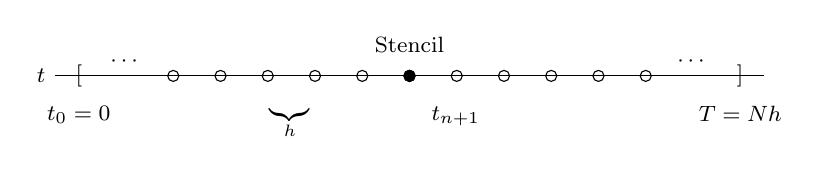
\begin{tikzpicture}
		  \labelnum[yshift=-2cm]{2}{Stencil}
		\end{tikzpicture}
	}
 	\only<3>{
		\begin{equation*}
			x(t_{n+1}) = 
			x(t_{n}) 
			+
			\int_{t_{n}}^{t_{n+1}} f(x(s),s)ds
		  +
		  \int_{t_{n}}^{t_{n+1}} g(x(s),s)dB(s)
		\end{equation*}
	}
	\only<4-6>{
		\begin{equation*}
			x(t_{n+1}) = 
			x(t_{n}) 
			+
			\underbrace{
				\int_{t_{n}}^{t_{n+1}} f(x(s),s)ds
		  }_{%
				  \textcolor<5-6>{red}{%
					  \approx \text{det}%
					 }
				}
		  +
		  \underbrace{
			  \int_{t_{n}}^{t_{n+1}} g(x(s),s)dB(s)
			}_{%
					\textcolor<6>{red}{%
						\hyperlink{frm:integracion}{\approx}
						%\approx
						}
				}
		\end{equation*}
	}
	\hypertarget<6>{frm:incremento_bm}{}
	\only<7->{
		\begin{equation*}
			x(t_{n+1}) = 
			x(t_{n}) 
			+
			\underbrace{
				\int_{t_{n}}^{t_{n+1}} f(x(s),s)ds
		  }_{%
				  \textcolor{red}{%
					  \approx 
					   f(x_n) h
					 }
				}
		  +
		  \underbrace{
			  \int_{t_{n}}^{t_{n+1}} g(x(s),s)dB(s)
			}_{
				\substack{
					\approx 
					g(x_n) \Delta B_n \\
					\Delta B_n = B_{t_{n+1}}-B_{t_n}
				}
			}
		\end{equation*}
	}
	\only<7>{
		\begin{textblock*}{.25\textwidth}(4.5cm,3.0cm)
			\begin{exampleblock}{}
				% left hand sums
				\centering
				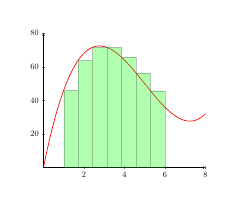
\begin{tikzpicture}[scale=0.3,%
				/pgf/declare function={f=-15*(x-5)+(x-5)^3+50;}]
					\begin{axis}[
					        xmin=0,xmax=8,ymin=0,ymax=80,
					    domain=0:10,
					    samples=100,
					    axis lines=middle
					]
					\addplot [thick, red] {f};
					\addplot [
					    black!80,fill=green,opacity=.3,
					    left segments=7,
					    left=1:6
					] {f};
					\end{axis}
				\end{tikzpicture}
			\end{exampleblock}
		\end{textblock*}
	}
 	\only<8>{
		\begin{align*}
				X_0 &=x_0, \qquad X_n  \approx x(t_n),
				\qquad 
				n=1 \dots, N-1
				\\
				X_{n+1} &= X_n + f(X_n) h + g(X_n) \Delta B_n, 
		 \end{align*}
	}
 	\only<9>{
 		\begin{align*}
 			X_0 &=x_0, \qquad X_n  \approx x(t_n),
 			\qquad 
 			n=1 \dots, N-1
 			\\
 			X_{n+1} &= X_n + f(X_n) h + g(X_n) 
 			\textcolor{blue}{%
 				\underbrace{\Delta B_n}_{%
 					\approx
 				}%
 			}%
 	 \end{align*}
 	}
\end{frame}

    \section{Brownian Motion}
        \begin{frame}{Random Walk}
	\centering
	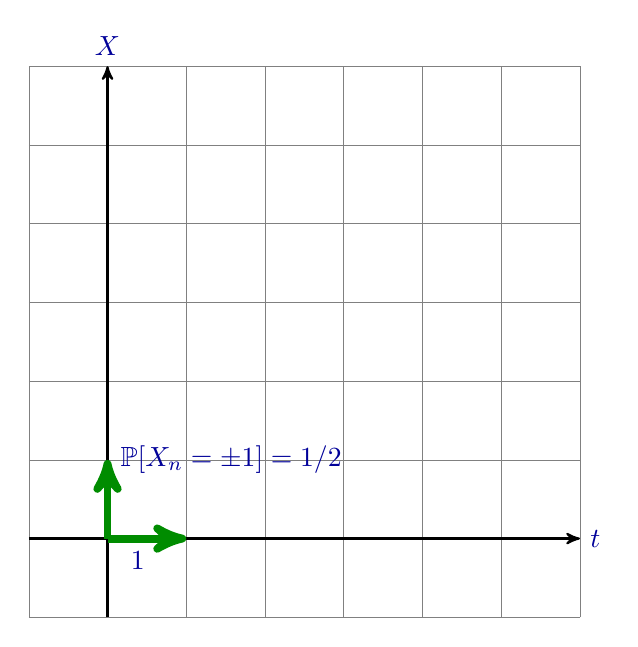
\begin{tikzpicture}[
    ,
    axis/.style={thick, ->, >=stealth'},
    pile/.style={%
    	line width=1.0mm,
        ->, 
        >=stealth', 
        color = black!45!green
    	},
    every node/.style={%
    	color=black!40!blue
	   }
    ]
    % axis
    \draw[step=1cm,gray,very thin] (-1,-1) grid (6,6);
    \draw[axis] (-1,0)  -- (6,0) node(xline)[right]
        {$t$};
    \draw[axis] (0,-1) -- (0,6) node(yline)[above] {$X$};
    % Lines
    \draw[pile] (0,0) coordinate (A) -- (0,1)
        coordinate (B) node[right, text width=10em] {$\P[X_n=\pm 1]=1/2$};
    \draw[pile] (0,0) coordinate (C) -- (1,0)
        coordinate (D) node[below, text width=4em] {1}; 
	\end{tikzpicture}
\end{frame}
%%%%%%%%%%%%%%%%%%%%%%%%%%%%%%%%%%%%%%%%%%
\begin{frame}{RandomWalk}
	\begin{overlayarea}{\textwidth}{.7\textheight}
	\only<1>{
	\begin{center}
		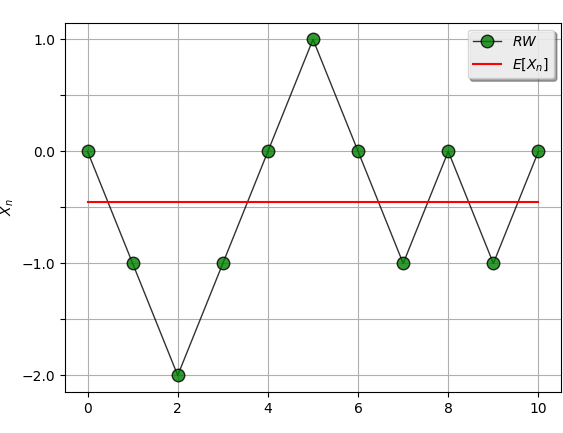
\includegraphics[width=.9\textwidth]{./IMAGENES/RW/RandomWalk(1).png}
	\end{center}
	}
	\only<2>{
		\begin{center}
			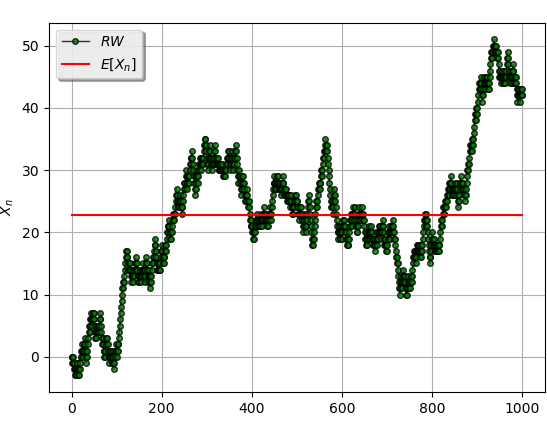
\includegraphics[width=0.83\textwidth]{./IMAGENES/RW/RandomWalk[2].png}
		\end{center}
	}
	\only<3>{
		\begin{center}
			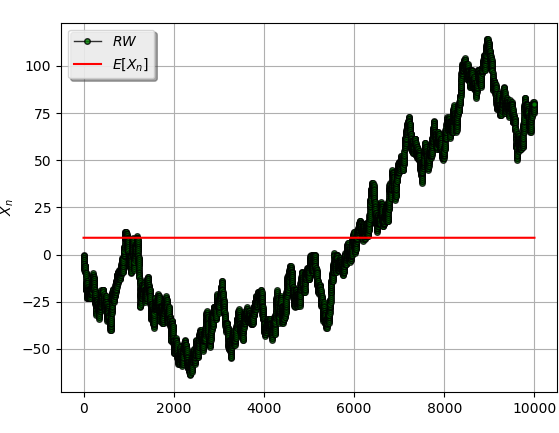
\includegraphics[width=0.83\textwidth]{./IMAGENES/RW/RandomWalk[3].png}
		\end{center}
	}
	\end{overlayarea}
\end{frame}
%%%%%%%%%%%%%%%%%%%%%%%%%%%%%%%%%%%%%%%%%%%%%%%%%%%%%%%%%%%%%%%%%%%%%%%%%%%%%%%%
%%%%%%%%%%%%%%%%%%%%%%%%%%%%%%%%%%%%%%%%%%%%%%%%%%%%%%%%%%%%%%%%%%%%%%%%%%%%%%%%
\begin{frame}{}
	\centering
	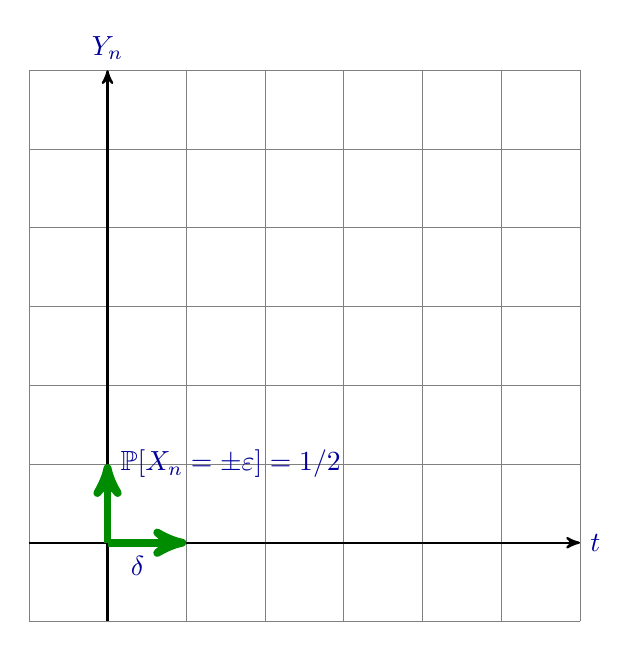
\begin{tikzpicture}[
    scale=1,
    axis/.style={thick, ->, >=stealth'},
    pile/.style={%
    	line width=1.0mm,
        ->, 
        >=stealth', 
        color=black!45!green
    	},
    every node/.style={%
    	color=black!40!blue
	   }
    ]
    \draw[step=1cm,gray,very thin] (-1,-1) grid (6,6);
    \draw[axis] (-1,0)  -- (6,0) node(xline)[right]
        {$t$};
    \draw[axis] (0,-1) -- (0,6) node(yline)[above] {$Y_n$};
    \draw[pile] (0,0) coordinate (A) -- (0,1)
        coordinate (B) node[right, text width=10em] {%
        $\P[X_n=\pm \varepsilon]=1/2$%
        };%
    \draw[pile] (0,0) coordinate (C) -- (1,0)
        coordinate (D) node[below, text width=4em] {$\delta$}; 
	\end{tikzpicture}
\end{frame}
%%%%%%%%%%%%%%%%%%%%%%%%%%%%%%%%%%%%%%%%%%%%%%%%%%%%%%%%%%%%%%%%%%%%%%%%%%%%%%%
\begin{frame}{}
	\begin{columns}
		\column[t]{.5\textwidth}
		\begin{overlayarea}{\textwidth}{\textheight}
			\only<2->{
				\begin{empheq}{align*}
					&\{ X_{n} \}_{n=1}^{\infty}   \quad  i.i.d\\
					& \probX{X_{j} = \pm \varepsilon} = \frac{1}{2}.
				\end{empheq}
			}
			\only<3->{
				\begin{empheq}[box=\shadowbox*]{align*}
					Y_{\delta, \varepsilon}(0) = &0\\
					Y_{ \delta, \varepsilon}(n \delta )= 
					&
					X_{1} + X_{2} + \cdots + X_{n}.
				\end{empheq}
			}
			\only<4->{
				\begin{empheq}{align*}
					Y_{\delta, \varepsilon}(t) =
						&
							\frac{(n + 1) \delta - t}{\delta} 
							Y_{\delta, \varepsilon} (n \delta)
						\\
					 +
					 &
						 \frac{t - n \delta}{\delta}
						 Y_{\delta, \varepsilon}
						\left(
							 (n+1) \delta
						\right).
					\\
					&
						n \delta < t < (n + 1) \delta .
				\end{empheq}
				}			
		\end{overlayarea}
	\column[t]{.6\textwidth}
		\begin{overlayarea}{\textwidth}{\textheight}
			\only<5->{
				\begin{alertblock}{We want}
					 $$
						\lim_{
							\substack{
								\delta\to 0\\
								\varepsilon \to 0
							}
						}
					 	Y_{\delta, \varepsilon}
					 $$
				\end{alertblock}
			}
			\only<6>{
				Let
		 		$
					\lambda \in \mathbb{R}
				$ fixed. Compute
		 		\\
		 		\hyperlink{dfn:FuncionCaracteristica}{\beamergotobutton{caracteristica}}
				$
					\displaystyle
					\lim_{\delta, \varepsilon \to 0}
					\mathbb{E}
					\left[
						e^{ 
							i \lambda 
							Y_{\delta, \varepsilon}(t)
						}
					\right]
				$.
				\\
				\hypertarget{cns:Limite}{}
			}
			\only<7->{
				\textcolor<7>{red}{$t=n\delta$},
			}
			\only<7>{
				\begin{align*}
					\EX{
						e^{
							i\lambda
							Y_{\delta, \varepsilon}(\textcolor{red}{t})
						}
					}
					&=
					\prod_{j=1}^{n}
					\EX{
						e^{%
							i \lambda X_{j}%
						}
					}
					\\
					&=
					\left( 
						\EX{
							e^{i\lambda X_{j}}
						}
					\right)^{n}
					\\
					&=
					\left(
						\frac{1}{2} 
							e^{i \lambda \varepsilon}
					+
						\frac{1}{2}
							e^{-i \lambda \varepsilon}
					\right)^{n}
					\\
					&=
					\left(
						\cos(\lambda \varepsilon)
					\right)^{n}\\
					&=
					\left(
						\textcolor{blue}{\cos(\lambda \varepsilon)}
					\right)^{
									\frac{t}{
										\textcolor{blue}{\delta}
									}
							}.
				\end{align*}
			}
			\only<8->{
				\textcolor{cyan}{
					$
						u =
						\left(
							cos(\lambda \varepsilon)
						\right)^{\frac{1}{\delta}}
					$
				}
			}
			\only<9-10>{
				$
					\ln(u)= \frac{1}{\delta} 
					\ln(cos(\lambda \varepsilon))
				$
				\\
				For $x,\epsilon$ small!
				$
					\ln(1+x)\approx x 
				$
				\\
				%
				$$
                    \cos(\lambda \epsilon)
					\approx 
					\underbrace{
                        1 - \frac{1}{2} \lambda^2 \varepsilon^2	
                    }_{1 + x}.
				$$
				Then
			}
			\only<11-12>{
				\begin{empheq}{align*}
					u \approx 
						& 
						e^{ 
							- \frac{1}{2\delta}
							\lambda^{2}
							\varepsilon^{2}
						}
					\\
					\EX{
						e^{ 
							i \lambda 
							Y_{\delta, \varepsilon}(t)
						}
					}
					\approx &
					e^{
						- \frac{1}{
								2
								\textcolor{red}{\delta}
						}
						 t\lambda^{2}
						\textcolor{red}{\varepsilon}^{2}
					}.
			\end{empheq}
			}
			\only<11->{
				\textcolor{red}{$\varepsilon^{2} = \delta$}
			}
			\only<11->{
				$$
					\displaystyle
					\lim_{
						\delta \to 0 
					}
					\EX{
						e^{
							i \lambda 
							Y_{\delta, \sqrt{\delta}} (t)
						}
					}
					= 
					e^{ 
						-\frac{1}{2} t 
						\lambda^{2}
					},
					\qquad \lambda \in \mathbb{R}.
				$$
			}	\only<12>{
		 			\begin{empheq}[box=\ovalbox]{equation*}
		 			\therefore
		 			B(t)
		     			\overset{ \mathcal{D} }{ = }
		   				\displaystyle
		   				\lim_{\delta \to 0}
								Y_{\delta, \sqrt{\delta}}(t)
		 			\end{empheq}
				}
			\end{overlayarea}
		\end{columns}
\end{frame}
%%%%%%%%%%%%%%%%%%%%%%%%%%%%%%%%%%%%%%%%%%%%%%%%%%%%%%%%%%%%%%%%%%%%%%%%%%%%%%%
\begin{frame}{Construction}
	\begin{theorem}
    
		Let $Y_{\delta, \varepsilon}(t)$ a random walk starting at $0$,
		with jumps $\varepsilon$ , $-\varepsilon$, of equal probability at
		$\delta, 2\delta,3\delta, \ldots $.
		Assume $\varepsilon^{2} = \delta$.
		Then for each $t \geq 0$, the limit
		$$ 
			B(t) = \displaystyle
			\lim_{\delta \to 0}
			Y_{\delta, \sqrt{\delta}}(t),
		$$
		exist in distribution, 
		$$
			\mathbb{E}\left[e^{i\lambda B(t)}\right]
				= e^{- \frac{1}{2}t\lambda^{2}}, \quad \quad \lambda \in 	\mathbb{R}.
		$$
	\end{theorem}
\end{frame}
%%%%%%%%%%%%%%%%%%%%%%%%%%%%%%%%%%%%%%%%%%%%%%%%%%
\begin{frame}{Code}
	\only<+>{
  	\begin{figure}
  	\centering
      \tiny
   	\lstset{language=python}
         \lstinputlisting[firstline=3,lastline=11]{RW01.py}
   \end{figure}
}
\end{frame}
%%%%%%%%%%%%%%%%%%%%%%%%%%%%%%%%%%%%%%%%%%%
\begin{frame}{}
	\begin{overlayarea}{\textwidth}{.7\textheight}
	\only<1>{
		\begin{center}
			\includegraphics[width=.85\textwidth,keepaspectratio]%
			{./IMAGENES/RW/RW01(1).png}
		\end{center}
	}
	\only<2>{
		\begin{center}
			\includegraphics[width=.85\textwidth,keepaspectratio]%
			{./IMAGENES/RW/RW01(2).png}
		\end{center}
	}
	\only<3>{
		\begin{center}
			\includegraphics[width=.85\textwidth,keepaspectratio]%
			{./IMAGENES/RW/RW01(3).png}
		\end{center}
	}
	\end{overlayarea}
\end{frame}
%%%%%%%%%%%%%%%%%%%%%%%%%%%%%%%%%%%%%%%%%%%%%%%%%%%%%%%%%%%%%%%%%%%%%%%%%
\begin{frame}{}
	\begin{empheq}[box={\Garybox[Construcci\'on]}]{align*}
		\varepsilon^{2} 
		& =
			\delta
		\\
		Y_{\delta, \varepsilon}(t)
		& 
			\xrightarrow[\delta, \varepsilon \to 0]{%
				\mathcal{D}
			} B(t) 
			\qquad \forall t 
			\geq 0
			\\
		\EX{
			e^{i\lambda B(t)}
		}
		&
		\xrightarrow{\delta ,\varepsilon \to 0}
			e^{
				-\frac{1}{2}t
				\lambda^{2}
			}, \quad \lambda \in 	\mathbb{R}.
	\end{empheq}
\end{frame}
%%%%%%%%%%%%%%%%%%%%%%%%%%%%%%%%%%%%%%%%%%%%%%%%%%
\begin{frame}{}
	\begin{figure}
		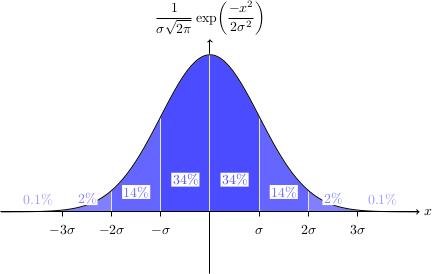
\includegraphics[width=\textwidth]{%
			./IMAGENES/RW/Standard_deviation_diagram.png%
		}
	\end{figure}
\end{frame}
%%%%%%%%%%%%%%%%%%%%%%%%%%%%%%%%%%%%%%%%%%%%%%%%%%%%%%%%%%%%%%%%%%%%%%%%%%
\begin{frame}{}
	%\vspace{-1.5cm}
	\begin{overlayarea}{\textwidth}{.7\textheight}
	\only<1>{
		\begin{center}
			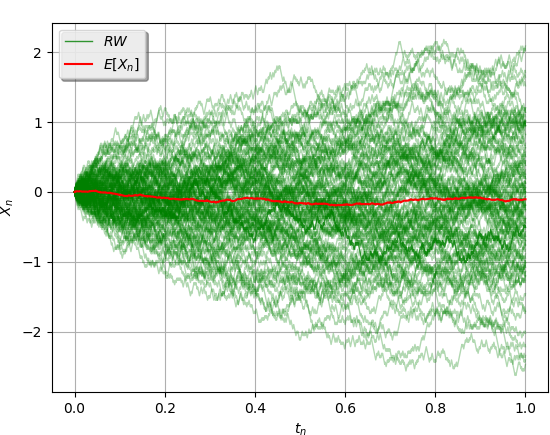
\includegraphics[width=.8\textwidth]{./IMAGENES/RW/RWs01.png}
		\end{center}
	}
	\only<2>{
		\begin{center}
			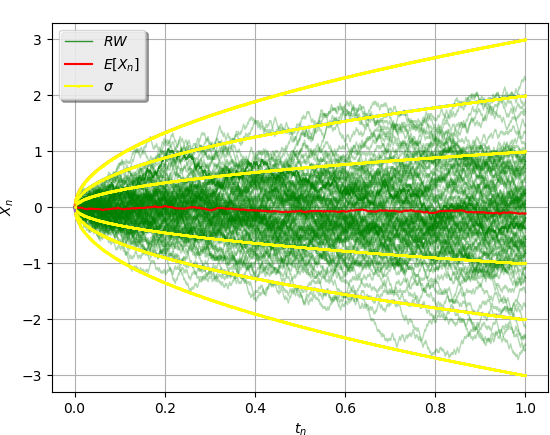
\includegraphics[width=.8\textwidth]{./IMAGENES/RW/RWs01Sigma.png}
		\end{center}
	}
	\end{overlayarea}
\end{frame}
%%%%%%%%%%%%%%%%%%%%%%%%%%%%%%%%%%%%%%%%%%%%%%%%%%%%%%%%%%%%%%%%%%%%%%%%%%%%%%%
\begin{frame}{Strong approximation}
	\begin{definition}
		Brownian motion B is the unique process that satisfies
		\begin{enumerate}[(i)]
			\item 
				$B(0)=0$ c.s.
			\item 
				\textcolor<6>{orange}{
					Para $0\leq s \leq t$,
					$
						B(t) - B(s) \sim \sqrt{t-s} N(0,1).
					$
				}
			\item
				for each $t_0 \leq t_1 \leq \dots \leq t_n \in [0,T]$, 
				r.v.  $B(t_i)- B(t_j)$  are independent 
		\end{enumerate}
	\end{definition}
	\begin{overlayarea}{\textwidth}{0.5\textheight}
		\only<2-4>{
			Then, given $t\in[0,T]$, and a stencil
			$$
				0=t_0 \leq t_1 \leq \cdots \leq t_{M-1} \leq t_{M}=t
			$$
			\only<3>{
				$$
					B(t) = \sum_{j=1}^M 
						B(t_j)-B(t_{j-1}).
				$$
			}
			\only<4>{
			$$
				B(t) = \sum_{j=1}^M 
					\underbrace{
						B(t_j)-B(t_{j-1}).
					}_{:=\Delta B_j}
			$$
			}
		}
		\only<5-6>{
			Let $\{t_n\}_{n=0}^N$, $t_n = nh$, 
			$$
				B(t_n) \approx 
					\sum_ {j=0}^n \Delta B_j, 
					\qquad
					\Delta B_0:=0,
					\qquad
					\only<6>{
						\textcolor{orange}{
							\Delta B_j \sim \sqrt{h} N(0,1).
						}
					}
			$$	
		}
	\end{overlayarea}
\end{frame}
%%%%%%%%%%%%%%%%%%%%%%%%%%%%%%%%%%%%%%%%%%%%%%%%%%%%%%%%%%%%%%%%%%%%%%%%%%%%%%%%

    \section{Weak vs Strong}
        \begin{frame}
  \frametitle{Weak vs Strong}
  \begin{empheq}[box={\Garybox[given]}]{align*}
 		dx(t)
			&=f(x(t))dt + g(x(t)) dB(t), 
 		\\
			x(0) &= x_0, \quad t\in[0,T]
 	\end{empheq}
  \begin{overlayarea}{\textwidth}{.7\textheight}
    \begin{columns}
      \column{.48\textwidth}
        \begin{block}{Weak}
          $$
						X_{n+1} = X_n + f(X_n) h 
							+ g(X_n) 
							\underbrace{\Delta B_n}_{%
								\substack{
									\approx \sqrt{h} \varepsilon_n\\
									\probX{\varepsilon_n=\pm 1}=1/2
								}
							}
					$$
        \end{block}
        %%%%%%%%%%%%%%%%%%%%%%%%%%%%%%%%
        \column{.48\textwidth}
          \begin{exampleblock}{strong}
          $$
						X_{n+1} = X_n + f(X_n) h 
							+ g(X_n) 
							\underbrace{\Delta B_n}_{%
								\substack{
									\approx \sqrt{h} \epsilon_n\\
									\epsilon_n \sim N(0,1)
								}
							}
					$$
          \end{exampleblock}
    \end{columns}
  \end{overlayarea}
\end{frame}
        \begin{frame}[plain,noframenumbering]
    \frametitle{Some representative schemes}    
    \begin{columns}
        \column{.3\textwidth}
            \begin{itemize}
                \item \structure<1-2>{\textbf{Implicite}:}
                    \begin{itemize}[<+-| alert@+>]
%                       \item
%                           SSEM
                        \item 
                            $\theta$-BEM
                        \item
                            FBEM
                    \end{itemize}
                \item \structure<3-5>{\textbf{Explicit}:}
                    \begin{itemize}[<+-| alert@+>]
                        \item 
                            Tamed EM 
                        \item
                            Truncated
                        \item
                            Sabanis
                    \end{itemize}
            \end{itemize}
        \column{.8\textwidth}
            \begin{overlayarea}{\textwidth}{.9\textheight}
                \only<1>{
                    \begin{bibunit}[alpha]
                        \begin{block}{$\theta$-Euler Maruyama \nocite{Mao2013}}
                            \begin{align*}
                                Y_{k+1} &= Y_k + h(1-\theta)f(Y_{k}) + 
                                \theta f(Y_{k+1}) +
                                g(Y_k)\Delta W_k,
                                \\ & \theta \in [0,1].
                            \end{align*}
                        \end{block}
                        \biblio{PhdThesisBib.bib}
                    \end{bibunit}
                }
                \only<2>{
                    \begin{bibunit}[alpha]
                        \begin{block}{Forward-Backward Euler Maruyama 
                            \nocite{Mao2013}}
                            \begin{align*}
                                Y_{k} &= Y_{k-1} + h(1-\theta)f(Y_{k-1}) + 
                                    \theta f(Y_{k}) +
                                    g(Y_{k-1})\Delta W_{k-1}
                                    \\ 
                                \widehat{Y}_{k+1} &= \widehat{Y_k} + hf(Y_{k}) 
                                + 
                                g(Y_k)\Delta W_k,
                                \qquad \theta \in [0,1].
                            \end{align*}
                        \end{block}
                        \biblio{PhdThesisBib.bib}
                    \end{bibunit}
                }
                \only<3>{
                    \begin{bibunit}[alpha]
                        \begin{block}{Tamed Euler Maruyama 
                            \nocite{Hutzenthaler2012a}}
                            \begin{align*}
                                Y_{k+1} &= Y_k + \frac{h f(Y_{k})}{1 +h 
                                \|f(Y_k)\|} + 
                                g(Y_k)\Delta W_k
                            \end{align*}
                        \end{block}
                        \biblio{PhdThesisBib.bib}
                    \end{bibunit}
                }
                \only<4>{
                    \begin{bibunit}[alpha]
                        \begin{block}{Truncated Euler Maruyama \nocite{Mao2015}}
                            \begin{align*}
                                Y_{k+1} &= Y_k + f_{\Delta}(Y_k) h + 
                                g_{\Delta}(Y_k)\Delta_{k},\\
                                f_{\Delta}(x)&:=
                                    \left(
                                        |x|\wedge 
                                        \mu^{-1}(h(\Delta))\frac{x}{|x|}
                                    \right),\\
                                g_{\Delta}(x)&:=
                                    \left(
                                        |x|\wedge 
                                \mu^{-1}(h(\Delta))\frac{x}{|x|}
                                    \right)
                            \end{align*}
                        \end{block}
                        \biblio{PhdThesisBib.bib}
                    \end{bibunit}
                }
                \only<5>{
                    \begin{bibunit}[alpha]
                        \begin{block}{Euler Maruyama with varying coefficients 
                            \nocite{Sabanis2015}}
                            \begin{align*}
                                Y_{k+1} &= Y_k + 
                                    \frac{h f(Y_{k}) + g(Y_k)\Delta W_k }
                                    {
                                        1 +k^{-\alpha} 
                                        \left(
                                            \|f(Y_k)\|
                                            +\|g(Y_k)\|
                                        \right)
                                    },
                                    \quad \alpha \in (0,1/2]  
                            \end{align*}
                        \end{block}
                        \biblio{PhdThesisBib.bib}
                    \end{bibunit}
                }
            \end{overlayarea}
    \end{columns}
\end{frame}
        \begin{frame}{SDE solvers}
    \begin{itemize}
        \item
            Julia:
            \href{http://docs.juliadiffeq.org/latest/}{juliadiffeq}
         \item
             Python:
             \begin{itemize}
                \item    
                    \href{%
                        https://pythonhosted.org/StochPy/userguide_doc.html
                    }{StochPy}
                \item
                \href{%
                    https://pypi.org/project/sdeint/
                }{sdeint}
                \item
                    \href{https://pythonhosted.org/PyS3DE/}{Py3DE}
             \end{itemize}             
         \item
             R:
             \begin{itemize}
                \item
                    \href{%                 
                https://www.rdocumentation.org/packages/sde/versions/2.0.15}{%
                sde}
                \item
                    \href{https://rdrr.io/cran/sde/src/R/sde.sim.R}{sde.sim.R}
                
             \end{itemize}
            \item
                MATLAB:
                \href{%
                    https://www.mathworks.com/help/finance/sde-objects.html}{%
                    SDE Models}
    \end{itemize}
 \end{frame}
    \section{Convergence and stability}
        \begin{frame}[label=Extension]
    \frametitle{Common hypothesis}    
    \begin{overlayarea}{\textwidth}{.1\textheight}
        \vspace*{-.25cm}
        \begin{empheq}[box=\shadowbox]{equation*}
            dy(t) = f(y(t)) dt + g(y(t)) dW_t, \quad Y_0=y_0.  \tag{EDE}
        \end{empheq}
    \end{overlayarea}
    %
    \tcbset{
        enhanced,
        colback=black!5!white,
        boxrule=0.4pt,
        colframe=black!65!black,
        fonttitle=\bfseries
    }
    \begin{overlayarea}{\textwidth}{.9\textheight}
        \begin{columns}
            \column{.4\textwidth}
                \only<2-3>{
                    \begin{tcolorbox}[drop lifted shadow, title=Drifft]
                        \begin{align*}
                            f &: \R^d \to \R^d, \\  
                            f &= 
                            \left(
                                f^{(1)}, \dots, f^{(d)}
                            \right),            
                        \end{align*}                    
                    \end{tcolorbox}
                }
            %
            \column{.4\textwidth}
                \only<3>{
                    \begin{tcolorbox}[drop lifted shadow, title=Difusion]
                        \begin{align*}
                            g&: \R^d \to \R^{d \times m},\\
                            g&= 
                                \left(
                                    g^{(i,j)}
                                \right)_{
                                    \substack{
                                        i \in \{1,\dots, d\}\\
                                        j \in \{1,\dots, m\}
                                    }
                                }  \\
                            W &= \left(
                            W^{(1)}, \dots, W^{(m)}             
                            \right)                 
                        \end{align*}
                    \end{tcolorbox}
                }
        \end{columns}
        %
        
        
        \only<4->{
            \begin{tcolorbox}[title=Hypothesis]
                \begin{itemize}    
                 \item[(EU-1)]<6-> 
                    \structure{Local Lipschitz} 
                    \qquad
                    \textcolor{black}{
                        \only<6->{
                            \textcolor<6-9>{cyan}{
                                $\forall R>0$,   
                            }
                        }
                        \only<7->{
                            \textcolor<7-9>{cyan}{
                                \  $\exists L_f=L_f(R)>0$
                            }
                        }
                        %\vspace*{-0.4cm}
                        \only<8->{
                            \textcolor<8-9>{red}{
                                $
                                    |f(u)-f(v)|^2
                                    \leq L_{f}|u-v|^2 
                                $                               
                            }       
                        }
                        \only<9->{
                            \qquad 
                            \textcolor<9>{cyan}{
                                $\forall \ u,v \in \R^d,  |u|\vee|v|\leq R$
                            }                       
                        }
                    }
                    %\vspace*{.4cm}
                \item[(EU-2)]<10->
                    \textcolor{black}{
                        \structure{Local Lipschitz}                
                        \only<10->{
                            \qquad
                            \textcolor<10-12>{cyan}{
                                $\exists L_g>0$
                            } 
                        }
                        \only<11->{
                            \\
                            \textcolor<11-12>{red}{
                                $|g(u)-g(v)|^2 \leq L_{g}|u-v|^2,$
                            }
                        }
                        \only<12->{
                            \qquad
                            \textcolor<12>{cyan}{
                                $ \forall u,v \in \R^d.$
                             } 
                        }
                    }
                \item[(EU-3)]<13->
                    \textcolor{black}{
                        \structure{Monotony}
                        \only<14->{ 
                            \textcolor<14-16>{cyan}{
                                $\exists$ $\alpha$, $\beta>0$
                            }
                        }
                        \only<15>{
                        \\
                            \textcolor<15>{red}{
                                $
                                    \innerprod{u}{f(u)} +\frac{1}{2}|g(u)|^2
                                    \leq \alpha +\beta |u|^2, 
                                $
                            }                           
                        }                       
                        \only<16->{
                            \\                              
                            \textcolor<16-17>{red}{
                                $
                                    \innerprod{u}{f(u)}+\frac{p-1}{2}|g(u)|^2 
                                    \leq \alpha + \beta |u|^2,
                                $
                            }                       
                        }
                        \only<17->{
                            \qquad
                            \textcolor<17>{cyan}{
                                $\forall u \in \R^d.$
                            }                   
                        }
                    }       
                \end{itemize}
            \only<18->{         
                \tcblower               
                $
                    \Rightarrow
                $
                \hyperlink{ExistenciaMao}{              
                    \beamerbutton{              
                        $
                        \exists ! \ y(t)                
                        $
                    }
                }           
            }       
        \end{tcolorbox}
    }
    \end{overlayarea}
\end{frame}
%%%%%%%%%%%%%%%%%%%%%%%%%%%%%%%%%%%%%%%%%%%%%%%%%%%%%%%%%%%%%%%%%%%%%%%%%%%%%%%%
% %
\begin{frame}{EM results}   
    \begin{textblock*}{90mm}(10mm, 10mm)    
        \begin{empheq}[box=\shadowbox*]{equation*}
            dy(t) = f(y(t)) dt + g(y(t)) dW_t, \quad Y_0=y_0.  \tag{SDE}
        \end{empheq}
    \end{textblock*}
      %
        \begin{textblock*}{60mm}(10mm, 40mm)
            \begin{tcolorbox}[left=1mm, title= Hypothesis]
                \begin{enumerate}[(H1)]
                    \item 
                    %\structure{(H-1)}
                        \scalebox{.7}{
                            \textcolor{black}{
                                $\forall R>0$,  $\exists \  C_R>0$
                            }
                        }
                        \\
                        \scalebox{.7}{
                            \textcolor{black}{
                            $   
                                |f(x)-f(y)|^2 \vee |g(x)-g(y)|^2 
                                \leq 
                                C_R|x-y|^2
                            $
                        }
                        }
                        \\
                        \scalebox{.7}{
                            \textcolor{black}{
                            $
                                \forall x,y\in \R^d 
                                |x|\vee |y|\leq R.
                            $
                            }
                        }
                        \\
                    \item
                        %\structure{(H-2)}
                        \scalebox{0.7}{
                            Para alg\'un $p>2$, $\exists \  A>0$ t.q.
                        }
                        \scalebox{0.7}{
                            \textcolor{black}{
                                \textcolor<2->{red}{
                                    $
                                        \displaystyle
                                        \EX{\sup_{0\leq t\leq 
                                            T}|\overline{Y}(t)|^p}
                                        \vee
                                        \EX{\sup_{0\leq t\leq T}|y(t)|^p} 
                                            \leq A.
                                    $
                                }
                            }
                        }
                 \end{enumerate} 
                \tcblower
                \hspace*{.25cm}
                \only<3->{
                    $   
                        \overline{Y}(t):=
                        Y_{\eta(t)} + (t-t_{\eta(t)}) f(Y_{\eta(t)}) 
                    $   
                    \\
                    \hspace*{1.0cm}
                    $
                        + g(Y_{\eta(t)})(W(t)-W_{\eta(t)}),\\
                    $
                    \hspace*{.25cm}
                    $
                        \eta(t):=
                        k, \text{ for } t\in[t_k,t_{k+1})
                    $
                }
            \end{tcolorbox}                        
         \end{textblock*}
        \only<4->{
            \begin{textblock*}{60mm}(70mm, 10mm)
                \includegraphics[width=1\linewidth]{%
             ./Imagenes/HighamConvergence/ContinuousExtension.eps}
            \end{textblock*}
        }
            \only<5->{
                \begin{textblock*}{45mm}(75mm, 60mm)
                    \begin{theorem}
                        EM converge
                        \begin{equation*}
                            \lim_{h\to 0}
                            \EX{\sup_{0\leq t\leq T}|\overline{Y}(t)-y(t)|^2}=0.
                        \end{equation*}
                    \end{theorem}
                \end{textblock*}
            }
            \only<2-3>{
                \begin{bibunit}[apalike]
                    \nocite{Higham2002b}
                    \biblio{PhdThesisBib.bib}
                \end{bibunit}
            }
\end{frame}
%%%%%%%%%%%%%%%%%%%%%%%%%%%%%%%%%%%%%%%%%%%%%%%%%%%%%%%%%%%%%%%%%%%%%%%%%%
        \begin{bibunit}[apalike]
  \begin{frame}%[label=frm:10]
    \frametitle{Definiciones y resultados previos}
    \nocite{KloedenPllaten}
    \biblio{BibliografiaTesis}
  \end{frame}
\end{bibunit}
%%%%%%%%%%%%%%%%%%%%%%%%%%%%%%%%%%%%%%%%%%%%%%%%%%%%%%%%%%%%%%%%%%%%%%%%%%%%%%%%
\begin{frame}
    \frametitle{consistency}
    \vspace{-1.0cm} 
    \begin{empheq}[box={\Garybox[EDE]}]{equation*}
        dy(t) = f(y(t)) dt + g(y(t)) dW_t, \quad Y_0=y_0  \tag{EDE}
    \end{empheq}        
    \vspace{-.45cm} 
    \begin{columns}
        \column{.3\textwidth}
            Let $Y^{h}$ a one step  $\max h$.      
        \column{.5\textwidth}
        \begin{empheq}[box=\shadowbox]{equation*}
            \varepsilon(h)= \mathbb{E}
          \left(
            |y(T)-Y^{h}(T)|
          \right)
        \end{empheq}        
    \end{columns}   
    \vspace{-.5cm}  
    \begin{overlayarea}{\textwidth}{.7\textheight}
    \only<+->{
      \begin{definition}[]
        $Y^{h}$  at times
        $
          \left(
            \tau
          \right)_{h}=
          \left\{
            \tau_{n}:n=0,1,\cdots
          \right\}
        $
        is \textcolor{red}{strong consistent},
        si $\exists \ C=C(h)\geq 0,\quad h_0$ s.t.
        $\textcolor{red}{\forall Y_n^{h}},n=1,2,\dots, N, \quad h\in(0,h_0)$
        \begin{itemize}[<+->]
          \item $\displaystyle \lim_{h\downarrow 0} C(h)=0$
          \item
          $
            \displaystyle
             \mathbb{E}
              \left(
                \left|
                  \mathbb{E}
                  \left(
                    \frac{Y_{n+1}^{h}-Y_n^{h}}{h}
                      \left|
                        \mathcal{F}_{\tau_n}
                      \right.
                  \right)
                -
                \textcolor{red}{
                    f\left(
                        Y_{n}^{h}
                  \right)
            }
                \right|^2
             \right)\leq C(h).
          $
          \item
            \renewcommand{\arraystretch}{1.5}%
            \scalebox{0.8}{% Scale by 50%
            $
              \mathbb{E}
              \left(
                \frac{1}{h}
                \left|
                Y_{n+1}^{h}-Y_{n}^{h}-
                \mathbb{E}
                \left(
                  \frac{Y_{n+1}^{h}-Y_n^{h}}{h}
                    \left|
                    \mathcal{F}_{\tau_n}
                \right.
              \right)
            -
            \textcolor{red}{
                g\left(
                    Y_{n}^{h}
                \right)
            }
            \Delta W_n
            \right|^2
          \right)\leq C(h).
         $ }
        \normalsize
        \end{itemize}
      \end{definition}
        }
    \end{overlayarea}
\end{frame}
%%%%%%%%%%%%%%%%%Convergencia%%%%%%%%%%%%%%%%%%%%%%%%
\begin{frame}
    \frametitle{}
    \vspace{-1.0cm} 
    \begin{empheq}[box={\Garybox[EDE]}]{equation*}
        dy(t) = f(y(t))dt + g(y(t)) dW_t, \qquad y_0=y(0)  %\tag{EDE}
    \end{empheq}        
    \vspace{-.45cm} 
    \begin{columns}
        \column{.3\textwidth}
            $Y^{h}$   a scheme with     $\max h$.      
        \column{.5\textwidth}
        \begin{empheq}[box=\shadowbox]{equation*}
            \varepsilon(h)= \mathbb{E}
          \left(
            |y(T)-Y^{h}(T)|
          \right)
        \end{empheq}        
    \end{columns}   
    \vspace{-.5cm}  
    \begin{overlayarea}{\textwidth}{.7\textheight}
     \only<+>{
      \begin{definition}%[Strong convergent]
        $Y^{h}$ \textcolor{red}{is strong convergent}  
        to $y$ if at final time $T$ 
        \begin{equation*}
          \lim_{h \downarrow 0}
          \mathbb{E}
          \left(
              |y(T) - Y^{h}(T)|
          \right)=0
        \end{equation*}
      \end{definition}
      }
    \only<+>{
      \begin{definition}[convergence order]
        $Y^{h}$
        \textcolor{red}{is strong convergent} 
            \textcolor{red}{with order $\gamma$},
         if $\exists \ C$
        independent from $h $ y $h_{0}$ s.t.
        \begin{equation*}
          \epsilon(h)=
          \mathbb{E}
          \left(
            |y(T)-Y(T)|
            \right)\leq C h^{\textcolor{red}{\gamma}} 
            \qquad\forall h\in 
            (0,h_0).
        \end{equation*}
      \end{definition}
      }
    \end{overlayarea}
\end{frame}
%%%%%%%%%%%%%%%%%%%%%%%%%%%%%%%%%%%%%%%%%%%%%%%
\begin{frame}
    \frametitle{}  
    \hypertarget{thm:ConsistenciaConvergencia}{}    
    %\vspace{-3.8cm}    
    \begin{empheq}[box={\Garybox[SDE]}]{equation*}
        dy(t) = f(y(t))dt + g(y(t)) dW_t, \qquad y_0= y(0) 
    \end{empheq}
    \begin{overlayarea}{\textwidth}{\textheight}
        \begin{theorem}
         Consistency implies convergence
        \end{theorem}
    \end{overlayarea}
\end{frame}
%%%%%%%%%%%%%%%%%%%%%%%%%%%%%%%%%%%%%%%%%%%%%%%%

    \appendix
        %%%%%%%%%%%%%%%%%%%%%%%%%%%%%%%%%%%%%%%%%%%%%%%%%%%%%%%%%%%%%%%%%%%%%%%%%%%%%%%%
\begin{frame}[label=ExistenciaMao,noframenumbering]
    \frametitle{Apendice A: Existencia y unicidad (condiciones locales)}        
    \begin{overlayarea}{\textwidth}{1.0\textheight} 
    \begin{columns}
        \column{.57\textwidth}
            \begin{theorem}
                 (EU-1)-(EU-3)              
                $\Rightarrow$ 
                $\exists ! \  \{y(t)\}_{t\geq 0}$, $\forall y(0)=y_0\in 
                \mathbb{R}^d$. 
                \\              
                 Further
                 $0<T<\infty$,
                \begin{itemize}[<+-|alert@+>]
                    \item               
                    $
                        \EX{y(T)}< 
                            \left(
                                |y_0|^2 +2\alpha T 
                            \right)\exp(2\beta T),
                    $
                    \item               
                    $\tau_n := \inf \{ t\geq 0 : |y(t)|>n\}$, $n\in \N$,         
           
                    \only<3->{
                        $$  
                            \textcolor<3>{red}{
                                \prob{[\tau_n\leq T]}
                                \leq \frac{
                                \left(
                                |y_0|^2 +2\alpha T 
                                \right)
                                \exp(2\beta T)
                                }{n},
                            }
                        $$ 
                    }   
                    \item<4>                    
                        $
                            \textcolor<4>{red}{
                                \EX{|y(t)|^p}
                                \leq
                                2^{\frac{p-2}{2}}
                                \left(
                                1 + \EX{|y_0|^p}
                                \right)e^{Cpt}.             
                            }
                        $           
                \end{itemize}           
            \end{theorem}
        \column{.5\textwidth}       
            \begin{bibunit}[apalike]        
                \cite{Mao2013}          
                \biblio{PhdThesisBib.bib}
            \end{bibunit}
    \end{columns}
        
    \hyperlink{Extension<4>}{
        \beamerreturnbutton{Extension}
    }
    \end{overlayarea}
\end{frame}

%%%%%%%%%%%%%%%%%%%%%%%%%%%%%%%%%%%%%%%%%%%%%%%%%%%%%%%%%%%%%%%%%%%%%%%%%%%%%%%%
\end{document}